\documentclass[main.tex]{subfiles}

\begin{document}

\chapter{Libre échange et protectionnisme}

\section{Théorie des échanges internationaux}
Différentes théories des échanges internationaux se sont succédées depuis le 16\up{ème} siècle, parmi ces dernières on retrouve:
        \begin{itemize}
                \item le \emph{mercantilisme}, un courant de la pensée économique contemporain de la colonisation du Nouveau Monde et du triomphe de la monarchie absolue, du 16\up{ème} au 18\up{ème} siècle en Europe, 
                \item Ricardo énonce en 1817 sa théorie des \emph{avantages comparatifs} qui corrige celle des \emph{avantages absolus} d’Adam Smith, tout pays gagne avec le libre échange,
                \item la théorie de Cantillon et Hume, le \emph{mécanisme d'équilibre automatique} des échanges. Dès qu'un pays dispose d'une balance commerciale positive, c'est à dire un revenu lié aux exportations plus important que le coût des importations, il va recevoir un afflux de métaux précieux. Le niveau des prix va alors augmenter selon la théorie quantitative de la monnaie. 
                \item Critique anti libérale, List 1841, exemple du \emph{blocus continental} avec l'Angleterre. Favorable au Zollverein
        \end{itemize}

        \begin{definition}[Mercantillisme]
                Ce courant met en avant le protectionnisme et la guerre, militaire comme commerciale. Les échanges internationaux sont perçus comme des jeux à somme nulle.
                Ses tenants prônent le développement économique par l'enrichissement des nations au moyen d'un commerce extérieur convenablement organisé en vue de dégager un excédent de la balance commerciale.
        \end{definition}

        \begin{definition}[Avantages absolus]
                Théorie selon laquelle un pays profite du libre-échange s’il se spécialise dans la production des biens pour lesquels il a un avantage absolu, énoncée par Adam Smith. Elle mène à une situation problématique: si un pays n’a d’avantage absolu pour aucun produit, il n’aurait pas intérêt à se lancer dans la spécialisation d’un produit en particulier, et aurait intérêt à garder ses frontières fermées au commerce international.
        \end{definition}

        \begin{definition}[Avantages comparatifs]
                Selon la théorie des avantages comparatifs, un pays gagne à se spécialiser dans la production des biens pour lesquels son avantage comparatif est le plus élevé, c'est-à-dire dont les coûts relatifs sont les plus bas, et à échanger les biens qu'il ne produit pas. C’est donc un argument pour le libre-échange: tous les pays peuvent gagner du libre-échange s’ils se spécialisent, qu'ils disposent d'avantages absolus ou non. Une boucle rétroactive positive peut également se mettre en place, en se spécialisant dans la production d'un bien les coûts liés à la production de ce bien dans le pays sont naturellement amenés à baiser, augmentant son avantage comparatif.
        \end{definition}

        \begin{definition}[Théorie quantitative de la monnaie]
                Loi comptable fondée sur la relation de causalité entre la quantité de monnaie en circulation et le niveau général des prix. 
                Si $P$ représente le niveau des prix, $T$ la production d'un économie, $M$ la quantité de monnaie en circulation dans cette économie et $V$ la vitesse de circulation de cette monnaie, alors cette loi avance que
                \[
                MV = PT
                .\] On considère en général que $V$ et $T$ sont fixes. Si cependant $V$ n'est pas stable on peut augmenter $M$ sans forcément augmenter $P$, c'est un des problèmes d'aujourd'hui, on ne parvient plus à créer d'inflation. 
        \end{definition}

        \begin{theorem}[Hecksher Ohlin Samuelson]
                         Aussi nommé théorème de l'allocation optimale des ressources par l'échange.
                         Chaque acteur des échanges internationaux a intérêt à se spécialiser dans la production pour laquelle il possède une meilleure dotation en facteurs, capital, travail, ressources, \textit{etc}. 
                 \end{theorem}
        Le modèle s'appuie sur les avantages comparatifs de Ricardo mais la conclusion est encore plus forte: les pays pauvres n'ont d'autres choix que de se concentrer sur les productions de main d'oeuvre à faible qualification, cela entraine une convergence de la rémunération des facteurs. 
                         Ce sont de plus les différences de dotation initiales en facteurs de production qui sont à l'origine des avantages spécifiques de chaque pays. \\

                         Ce théorème permet dans une certaine mesure d'expliquer la mondialisation, il montre cependant que cela entraine une augmentation des écarts de salaires entre travaux qualifiés et travaux non qualifiés dans les pays développés. Si on note $w_{q}$ le salaire d'un travail, qualifié dans un pays donné et $w_{nq}$ le salaire d'un travail non qualifié, avec une minuscule lorsque la demande est plus faible que le nombre de travailleurs et une majuscule dans le cas inverse la figure \ref{fig:wages} illustre ce phénomène. \\

        \begin{figure}[htpb]
                \centering
                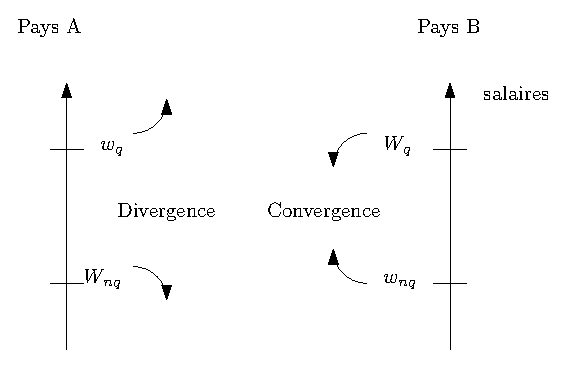
\includegraphics[width=0.8\textwidth]{wages.eps}
                \caption{Evolution des salaires dans un pays développé A et un pays en développement B}
                \label{fig:wages}
        \end{figure}

        Cela crée une forte dichotomie entre la moyenne mondiale du salaire d'un métier donné et le pouvoir d'achat au sein d'un pays. C. Freeman, expose ce problème dans son ouvrage \textit{Are your wages set in Beijing?}
        On pourrait penser que la délocalisation est l'unique facteur dans cette convergence, ce n'est pas forcément le cas, par exemple seulement 20\% du chômage lui est directement lié dans les pays développés.

        \subsection{Interrogation sur la théorie des échanges internationaux}

        Paradoxe de Leontief, USA taux de capital par tête est parmi les plus élevés, mais ils exportent des produits relativement intensifs en travail. Aux États Unis plus qu'ailleurs, le travail qualifié peut être considéré comme du capital (Keesing, 1966, puis jthéorie du capital humain de Becker)

        Enquêtes empiriques, prédictibilité HOS 60\%

        Maurice Allais
        Le protectionnisme entre pays à salaires comparables n'est pas souhaitable en général, celui entre pays de niveau de vie très différents est non seulement justifié mais absolument nécessaire.

        Années 1985/1990 Paul Krugman: Nouvelle théorie du Commerce International
        contexte: crise économique US dans les années 1980, nippophobie

        Observations: échanges plus denses entre pays équivalents en termes de facteurs de production, plus d'échanges intra branches que d'échanges inter branches

Explication: rendements croissants et concurrence imparfaite, accident historique explique le choix de produits de spécialisation
Krugman \textit{`La position extrême en faveur du libre échange est devenue intenable'}.

\begin{definition}[Effet de \textit{lock in}]
       Pays atteint une bonne position dans un oligopole, ou crée son propre monopole, il va le conserver pendant une longue période.
\end{definition}

\begin{definition}[Rendements croissants]
       Explique la plupart des monopoles. 
\end{definition}

        \section{Les gagnants et les perdants de la mondialisation}

        \subsection{Un processus continu}
        mise en relation ancien et nouveau monde, 16\up{ème} siècle
        19\up{ème}, le capitalisme industriel, Londres devient une nouvelle économie monde
        Après 1945, la mondialisation financière, le centre du monde se déplace vers les États Unis
        1980, accélération de la mondialisation dans une économie monde devenue numérique


        Une révolution des transports (Caravelle au 16\up{ème}, porte conteneurs au 19\up{ème}) et des moyens de communication
        La diffusion de politiques libérales en faveur de la libre circulation des marchandises, des services, des capitaux, et des hommes
        1995 OMC, 4 mondialisation Chine, \textit{etc.}

        Les importations de marchandises en dollars de différents pays

        \subsection{Bienfaits de la mondialisation}

        Avantage comparatif, coûts de production plus faibles, les consommateurs profitent de prix plus bas

        La libéralisation des échanges facilite la spécialisation internationale de la production

        Conséquences négatives
        Coûts d'ajustement élevé, délocalisation d'entreprises (direct), développement des importation évince les productions locales (indirect)
        UE met en place fond \ldots
        Forte instabilité financière
        Opposée à une croissance économique durable
        Effets de contagion, les mouvements boursier américains ont entrainé dans leur chute les marchés européens
        Crise de la dette souveraine.

        \subsection{Gagnants et perdants}
        
        Phénomènes inégalitaires avérés sur le long terme.
        Niveau de vie des pays les plus riche aujourd'hui 60 fois plus élevé que celui des pays moins développés.

        Inégalités entre individus
        main d'oeuvre qualifiéd des pays les plus développés et les détenteurs de capitaux bénéficient le plus de l'ouverture et leurs économies aux échanges 
\end{document}
